% \subsection{Appendix 1 - Toy Problem}

% \subsubsection{Discrete Case - Transition Matrix} \label{annexTransMat}




% \subsection{Appendix 2 - Case Study}
\subsection{Appendix 1 - Case Study}

\subsubsection{Load Case} \label{annexLoad}

To begin with, it should be mentioned that the calculations of the applied loads are made in an approximate fashion, since the case study is not an existing structure, meaning that any assumption could be justified as valid. This section aims to describe the step-by-step procedure of load calculation even for a real life application.\\

The elastic quasi-static forces per floor of the frame will be calculated according to the provisions of Eurocode 8 and the elastic response spectra. Using Equations (3.2) - (3.5) provided in Clause 3.2.2.2 of EN1998-1 \cite{EC8}, and the values included in Table \ref{spec1params}, the elastic response spectrum can be drawn\footnotemark.

\footnotetext{It is assumed that for the current application the ground type is $C$}

\begin{table}[H]
    \centering
    \caption{Values of the parameters describing the recommended Type I elastic response spectra \cite{EC8}}
    \label{spec1params}
    \begin{tabular}{ccccc}
        \toprule
        \textbf{Ground type} & $\boldsymbol{S}$ & $\boldsymbol{T_B(s)}$ & $\boldsymbol{T_C(s)}$ & $\boldsymbol{T_D(s)}$ \\
        \midrule
        A & $1.00$ & $0.15$ & $0.4$ & $2.0$ \\
        B & $1.20$ & $0.15$ & $0.5$ & $2.0$ \\
        C & $1.15$ & $0.20$ & $0.6$ & $2.0$ \\
        D & $1.35$ & $0.20$ & $0.8$ & $2.0$ \\
        E & $1.40$ & $0.15$ & $0.5$ & $2.0$ \\
        \bottomrule
    \end{tabular}
\end{table}

From the eigenanalysis of the frame, the eigenfrequencies are derived, with the fundamental one being $f_1 = 4.42 \, \mathrm{Hz}$, meaning that the fundamental period is $T_1 = 0.226 \, \mathrm{sec}$. Based on this period, and the drawn elastic response spectrum, the design ground acceleration is derived $S_{a,\,\text{el}} = 6.769 \, \mathrm{m/s^2}$ as illustrated in Figure \ref{elSpec}. 

\begin{figure}[H]
    \centering
	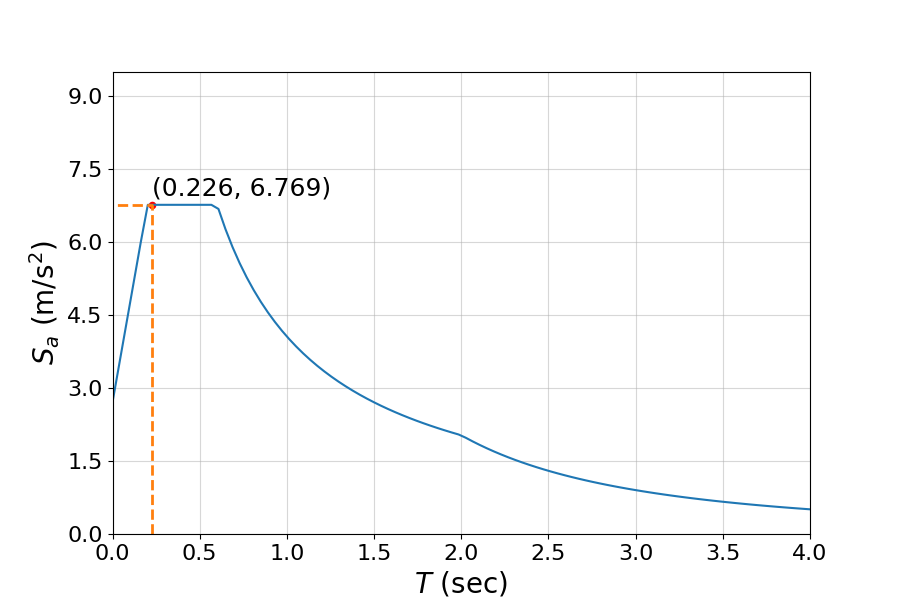
\includegraphics[width=0.6\linewidth]{Figures/elasticSpectrumAg.png}
	\caption{Elastic response spectrum}
	\label{elSpec}
\end{figure}

A simplified mass model for the frame is presented in Figure \ref{simpleFrame}, where $M$ represents the mass of the two columns and the beam of each floor. In particular, accounting for structural steel's mass density, $\rho = 7850 \, \mathrm{kg/m}^3$ and the geometric dimensions of the members (cross-sectional area and length), $M$ is calculated to be $1250\, \mathrm{kg}$.  Following this assumption, that the mass per floor is concentrated, the elastic quasi-static forces, are calculated as follows:

\begin{equation}
    F_{\text{el}\,,i} = S_{a, \,\text{el}}\, \Gamma \, m_i \, \varphi _i 
\end{equation}

where,
$$
\begin{aligned}
&m_{i}=\text { mass at floor } i \,\, [\mathrm{kg}] \\
&\varphi_{i}=\text { first eigenvector value, corresponding to floor } i\,\,[-] \\
&\Gamma = \text{ modal participation factor,} \quad \frac{\sum \varphi_{i} \cdot m_{i}}{\sum \varphi_{i}^{2} \cdot m_{i}}\quad[-] \quad (\text { for a diagonal mass matrix } \mathrm{M})
\end{aligned}
$$

The first eigenvector is plotted also in Figure \ref{simpleFrame}.

\vspace{0.2cm}

\begin{equation*}
    \varphi =
    \begin{Bmatrix}
        0.33\\
        0.66\\
        1.00
    \end{Bmatrix}
    \quad , \quad
    \underline{\underline{M}} =
    \begin{bmatrix}
    1250 & 0 & 0 \\
    0 & 1250 & 0 \\
    0 & 0 & 1250 \\
    \end{bmatrix}
    \quad , \quad 
    \Gamma = 1.288
\end{equation*}

\vspace{0.5cm}

\newpage

The needed quantities to calculated the quasi-static forces are included in Table \ref{elasticForces}.

\begin{table}[H]
    \centering
    \caption{Elastic quasi-static forces based on EN1998-1 \cite{EC8}}
    \label{elasticForces}
    \begin{tabular}{cccccc}
        \toprule
        \textbf{Floor, i} & $\boldsymbol{\phi _{i}}$ & \textbf{Floor mass} & $\boldsymbol{\Gamma }$ & $\boldsymbol{S_{a,\,\text{el}}}$ & $\boldsymbol{F_{\text{el,}\,i}}$ \\
        {[}-{]} & {[}-{]} & {[}kg{]} & {[}-{]} & {[}m/sec$^2${]} & {[}kN{]} \\
        \midrule
        1 & $0.33$ & $1250$ & $1.288$ & $6.769$ & $3.6$ \\
        2 & $0.66$ & $1250$ & $1.288$ & $6.769$ & $7.2$ \\
        3 & $1.00$ & $1250$ & $1.288$ & $6.769$ & $10.8$ \\
        \bottomrule
    \end{tabular}
\end{table}

\begin{figure}[H]
    \centering
	\makebox[\textwidth][c]{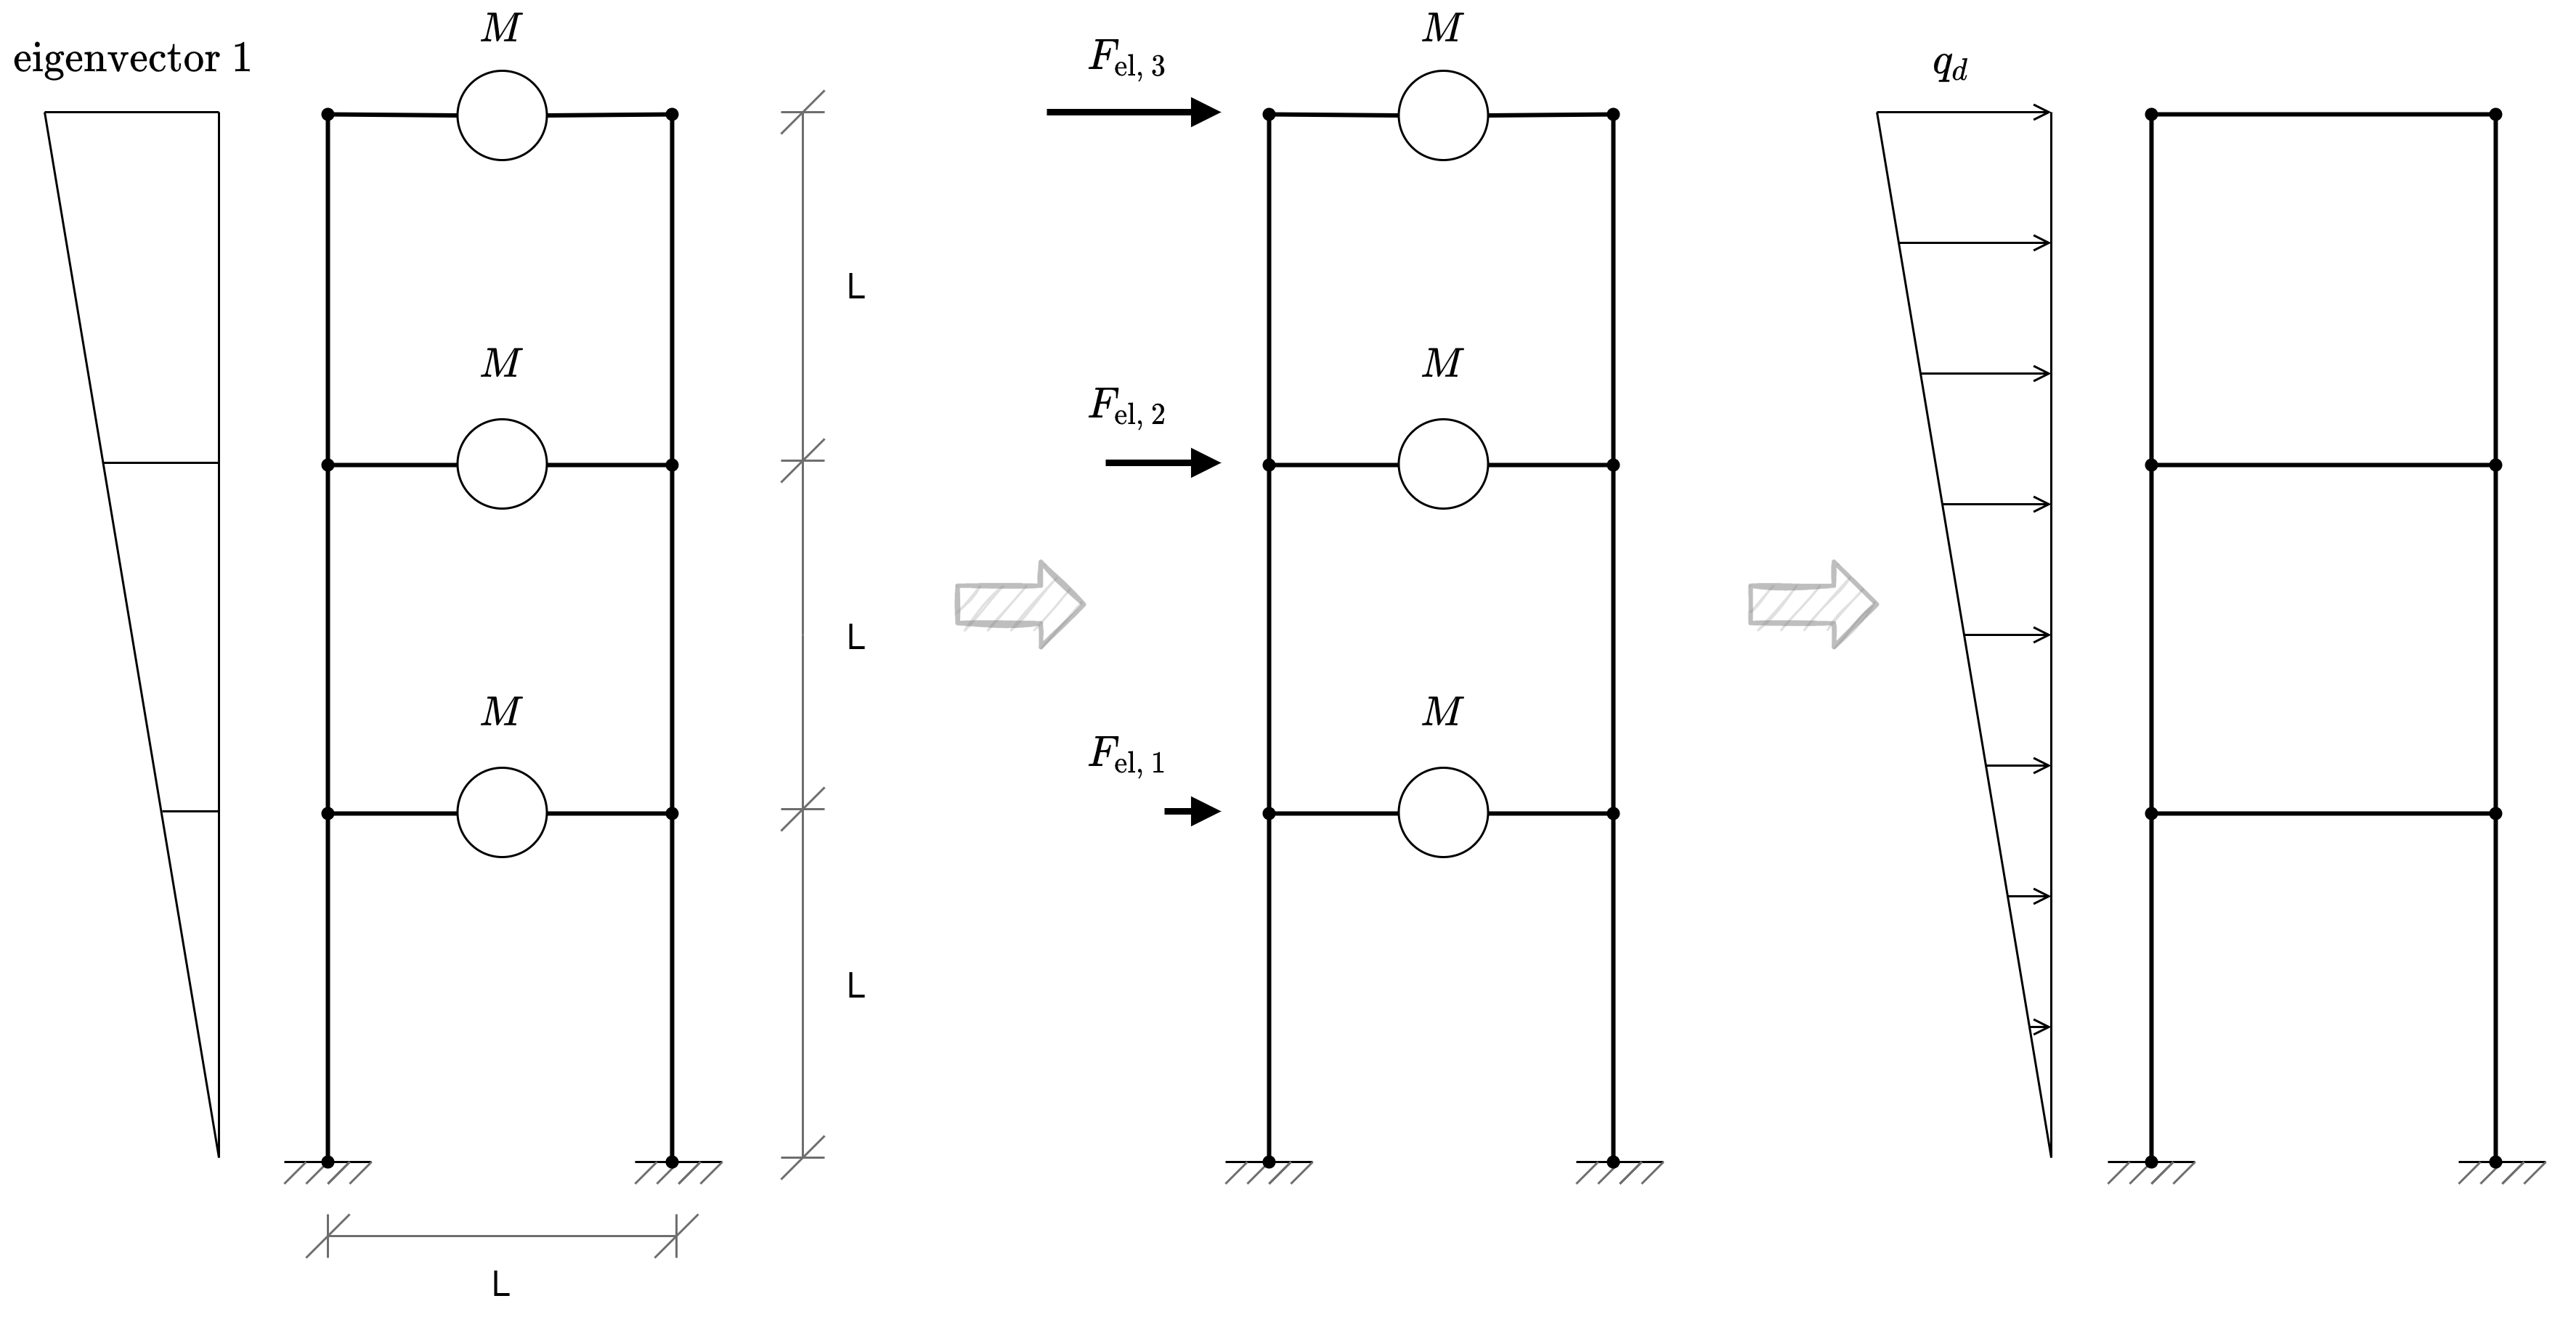
\includegraphics[width=1.1\linewidth]{Figures/simpleModel.png}}
	\caption{Simplified model of the frame}
	\label{simpleFrame}
\end{figure}


The superposition of these three concentrated loads will be now transformed into a triangular one, of value $q_d$ at the top node, as depicted also in Figure \ref{simpleFrame}.

\begin{gather}
    \sum _{i=1}^3 F_{\text{el,}\,i} = \frac{1}{2} \, 3 \, L \, q_d \nonumber\\
    \Rightarrow q_d = 3.6 \, \mathrm{kN/m}
\end{gather}

\newpage

\subsubsection{Deterioration} \label{annexDeter}

In the current project, the damage $d(\tau)$ is defined as the cross section loss, i.e. the ratio of the current cross-section area at deterioration rate $\tau$, over the initial one.

$$d(\tau) = \frac{A(\tau)}{A_0}$$

However, from a more pragmatic point of view, the damage, which is usually a reduction in thickness does not affect in the same way the flexural and the bending stiffnesses. The correlation between these two reductions is elaborated in this section.\\

Denoting as $c$ the corrosion penetration depth, and assuming that it is constant along the perimeter of the cross-section (Figure \ref{deterCrosSec}), the initial stiffnesses are:

\begin{gather}
    A_0 = 2 \, t_f \, b_f + t_w \, h_w \\
    I_0 = 2 \big[ \frac{1}{12}\, b_f \, t_f^3 + b_f\, t_f \, (\frac{h_w + t_f}{2})^2\big] + \frac{1}{12}\,t_w\,h_w^3
\end{gather}

where $t_f, b_f$ are the thickness and the width of the flange, and $t_w, h_w$ are the thickness and the height of the web, as displayed in Figure \ref{IPEgeom}.\\

\begin{figure}[H]
    \centering
	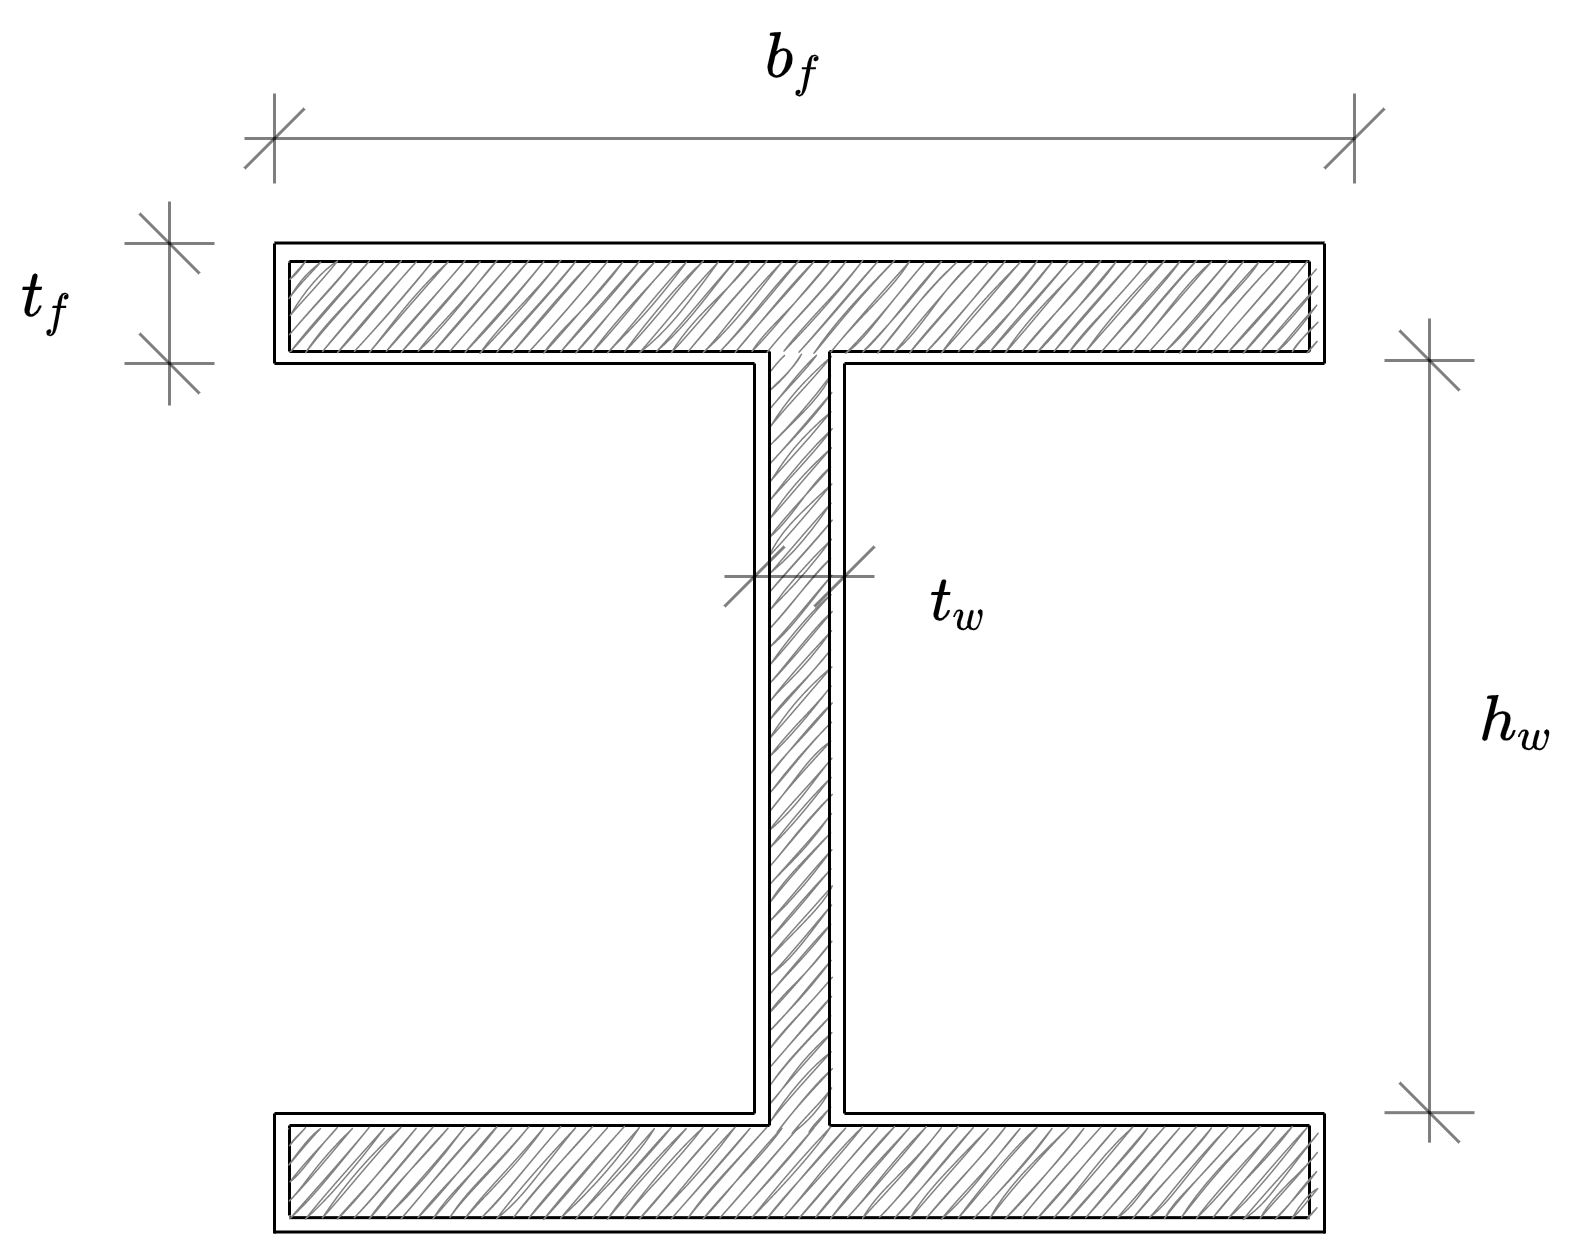
\includegraphics[width=0.5\linewidth]{Figures/IPEgeom.png}
	\caption{I-beam cross-section}
	\label{IPEgeom}
\end{figure}

The degraded cross-sectional area is:

\begin{equation}
    A = 2\, (t_f - 2\, c) \, (b_f - 2\, c) + (t_w - 2\,c)\,(h_w+2\,c) \label{AEq}
\end{equation}

\newpage

Subsequently, it holds:

\begin{gather}
    A_0 \, d = A \nonumber \\ 
    \Rightarrow \big[ 2 \, t_f \, b_f + t_w \, h_w \big] \, d = 2\, (t_f - 2\, c) \, (b_f - 2\, c) + (t_w - 2\,c)\,(h_w+2\,c) \nonumber \\ 
    \Rightarrow 4 \, c^2 + 2\,c\,(t_w-h_w - 2\,t_f - 2\,b_f) + (1 - d)\, \big[ 2 \, t_f \, b_f + t_w \, h_w \big] = 0 \nonumber \\ 
    \Rightarrow c = \cfrac{- 2\,(t_w-h_w - 2\,t_f - 2\,b_f) \pm \sqrt{\big(2\,(t_w-h_w - 2\,t_f - 2\,b_f)\big)^2 - 16\,(1 - d)\, \big(2 \, t_f \, b_f + t_w \, h_w \big)}}{8} \label{cEq}
\end{gather}

Then based on this value of corrosion penetration depth, $c$, the degraded moment of inertia is:

\begin{equation}
    I = 2 \, \Big[ \frac{1}{12}\, (b_f - 2\,c)\,(t_f-2\,c)^3 + (b_f-2\,c)\,(t_f-2\,c)\,\big( \frac{h_w+t_f}{2} \big) ^2 + \frac{1}{12}\,(t_w-2\,c)\,(h_w+2\,c)^3 \Big] \label{IEq}
\end{equation}

Concluding, using Equations \ref{cEq}, \ref{AEq}, \ref{IEq}, the degraded stiffnesses are calculated based on the damage of every decision step.